\documentclass[12pt]{article}
\usepackage[margin=1in]{geometry}
\usepackage{titling}
\usepackage[T1]{fontenc}
\usepackage{tabularx}
\usepackage{graphicx}
\usepackage{amsmath}

\pretitle{\begin{center}\Huge\bfseries}
\posttitle{\par\end{center}\vskip 0.5em}
\preauthor{\begin{center}\Large}
\postauthor{\end{center}}
\predate{\par\large\centering}
\postdate{\par}

\title{Algorytmy Metaheurystyczne - lab 0}
\author{Jakub Musiał 268442}
\date{Październik 2023}

\begin{document}

\maketitle

\hspace{1cm}

\section*{Cykl komiwojażera - algorytm MST}

\subsubsection*{Opis algorytmu}
    \begin{itemize}
        \item Wyznacz minimalne drzewo rozpinające za pomocą algorytmu Prima
        \item Wygeneruj cylk komiwojażera poprzez wyznaczenie kolejności odwiedzania
              wierzchołków grafu w algorytmie przeszukiwania w głąb
    \end{itemize}

    \noindent \newline

\subsubsection*{Wyniki}
    Poniższe table przedstawiają uzyskane wyniki, w tym wagę MST oraz TSP,
    a także minimalne wagi losowych cykli.

    \begin{table}[h!]
        \centering
        \begin{tabularx}{0.4935\textwidth}{| c | c | c |}
            \hline
            Dane wejściowe & Waga MST & Waga TSC \\
            \hline
            bcl380 & $1419$ & $2337$ \\
            pbk411 & $1157$ & $1930$ \\
            pbl395 & $1097$ & $1893$ \\
            pbm436 & $1238$ & $2095$ \\
            pbn423 & $1180$ & $1921$ \\
            pka379 & $1117$ & $1799$ \\
            pma343 & $1143$ & $1876$ \\
            xqf131 & $463$  & $742$  \\
            xqg237 & $878$  & $1424$ \\
            xql662 & $2193$ & $3692$ \\
            \hline
        \end{tabularx}
        \caption{Waga MST oraz TSP dla zadanych zestawów punktów}
        \label{table:weights}
    \end{table}

    \begin{table}[h!]
        \centering
        \begin{tabularx}{0.81\textwidth}{| c | c | c | c |}
            \hline
            Dane wejściowe & $min$ & $avg_{\text{min per 10 permutations}}$ & $avg_{\text{min per 10 permutations}}$ \\
            \hline
            bcl380 & $23545$ & $24503$ & $24111$ \\
            pbk411 & $20582$ & $21455$ & $21063$ \\
            pbl395 & $18353$ & $19054$ & $18746$ \\
            pbm436 & $21554$ & $22275$ & $21937$ \\
            pbn423 & $21311$ & $21782$ & $21473$ \\
            pka379 & $32344$ & $35091$ & $34023$ \\
            pma343 & $32444$ & $34239$ & $33349$ \\
            xqf131 & $4045$ & $4312$ & $4170$ \\
            xqg237 & $10681$ & $11749$ & $11452$ \\
            xql662 & $49641$ & $50872$ & $50210$ \\
            \hline
        \end{tabularx}
        \caption{Minimalne wagi losowych cykli dla zadanych zestawów punktór}
        \label{table:min_weights}
    \end{table}

    \newpage
    \noindent Można zauważyć, że generowanie cykli jako losowe permutacje zbioru wierzchołków daje
              zdecydowanie gorsze wyniki.

    \noindent \newline


\subsubsection*{Wizualizacja rozwiązań}

\begin{figure}[h]
    \centering
    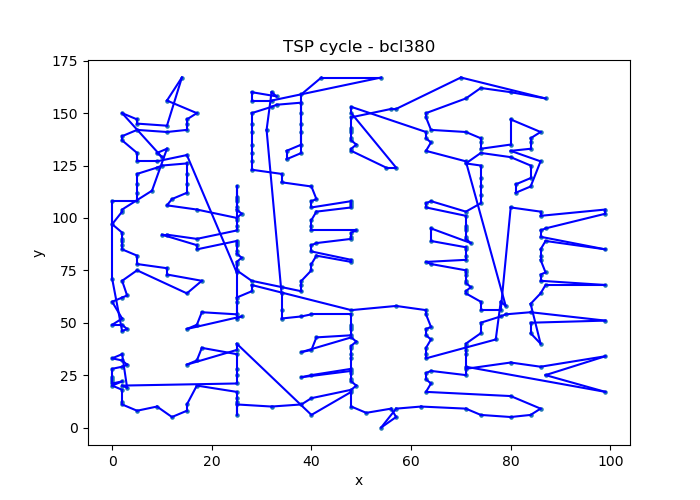
\includegraphics[width=0.8\linewidth]{img/bcl380.png}
    \label{fig:bcl380}
\end{figure}

\begin{figure}[h]
    \centering
    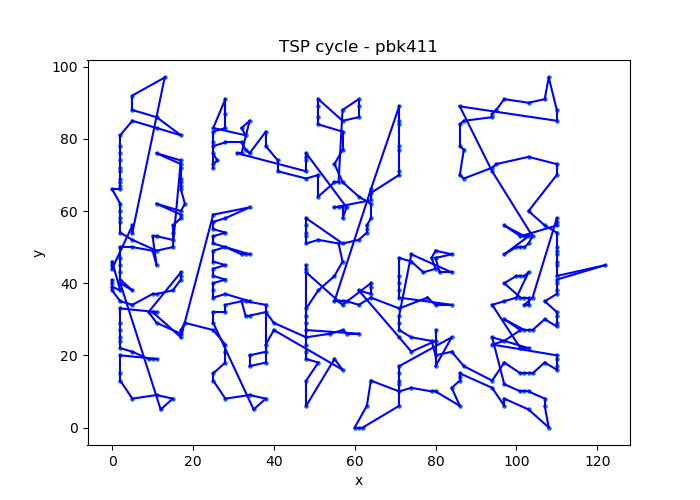
\includegraphics[width=0.8\linewidth]{img/pbk411.png}
    \label{fig:pbk411}
\end{figure}

\begin{figure}[h]
    \centering
    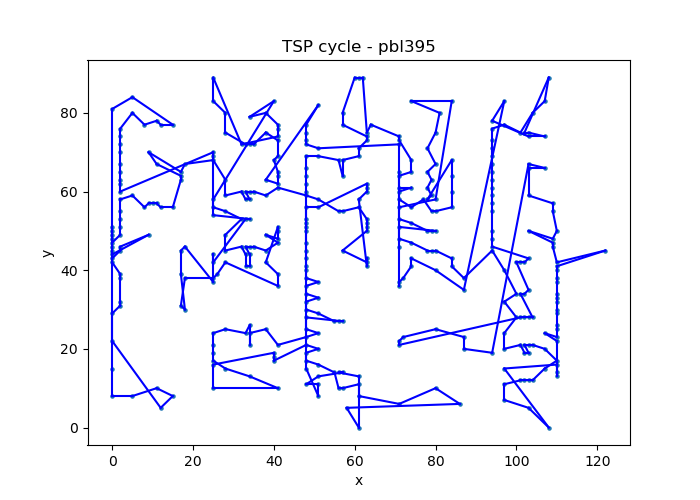
\includegraphics[width=0.8\linewidth]{img/pbl395.png}
    \label{fig:pbl395}
\end{figure}

\begin{figure}[h]
    \centering
    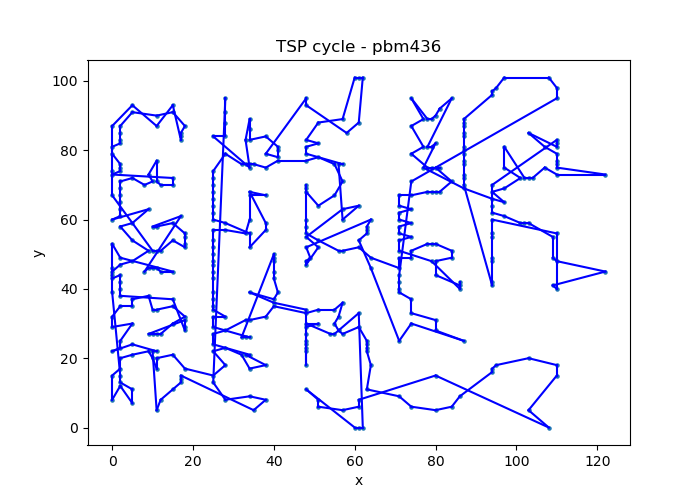
\includegraphics[width=0.8\linewidth]{img/pbm436.png}
    \label{fig:pbm436}
\end{figure}

\begin{figure}[h]
    \centering
    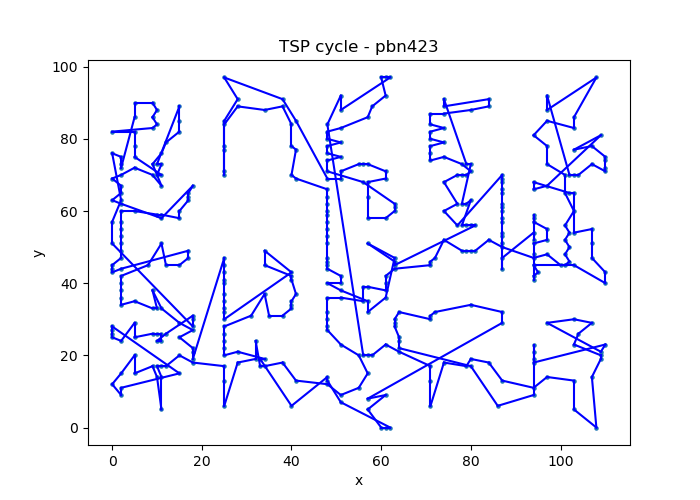
\includegraphics[width=0.8\linewidth]{img/pbn423.png}
    \label{fig:pbn423}
\end{figure}

\begin{figure}[h]
    \centering
    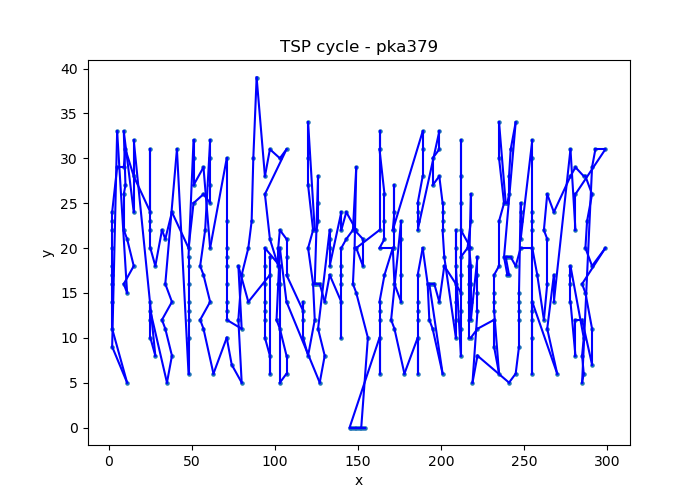
\includegraphics[width=0.8\linewidth]{img/pka379.png}
    \label{fig:pka379}
\end{figure}

\begin{figure}[h]
    \centering
    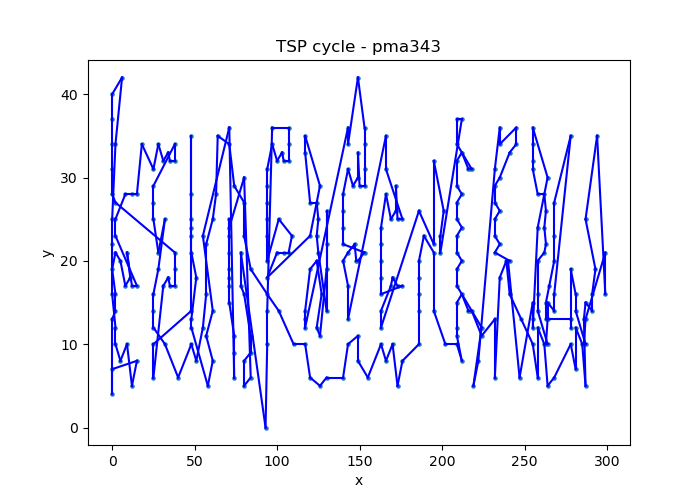
\includegraphics[width=0.8\linewidth]{img/pma343.png}
    \label{fig:pma343}
\end{figure}

\begin{figure}[h]
    \centering
    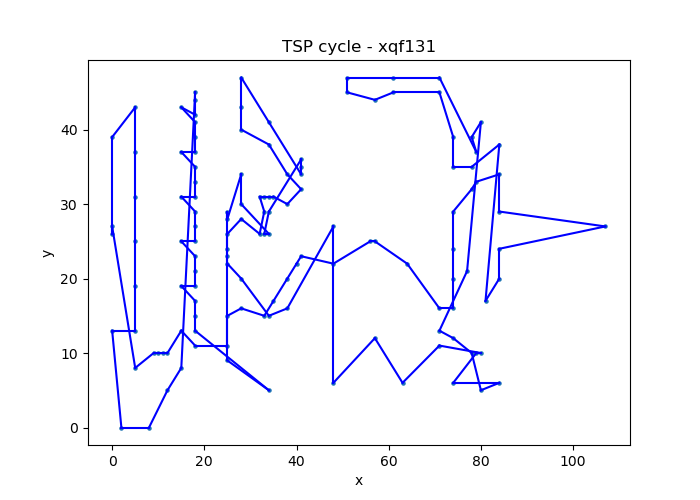
\includegraphics[width=0.8\linewidth]{img/xqf131.png}
    \label{fig:xqf131}
\end{figure}

\begin{figure}[h]
    \centering
    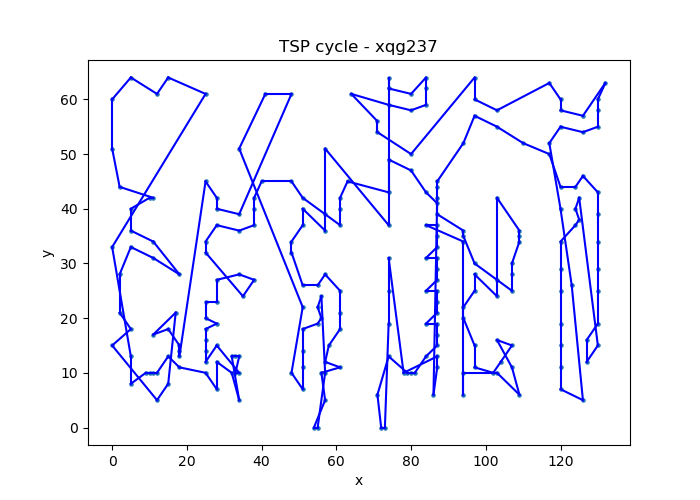
\includegraphics[width=0.8\linewidth]{img/xqg237.png}
    \label{fig:xqg237}
\end{figure}

\begin{figure}[h]
    \centering
    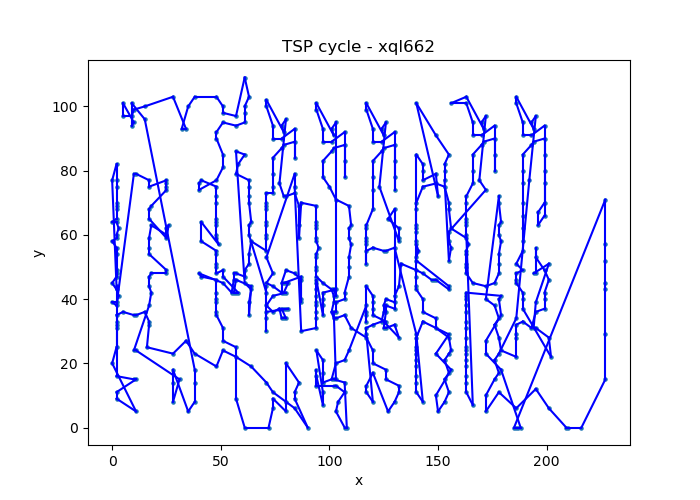
\includegraphics[width=0.8\linewidth]{img/xql662.png}
    \label{fig:xql662}
\end{figure}

\end{document}
